\section{Quark/Antiquark gluon emission kernel}


\begin{figure}[ht!]
\centering
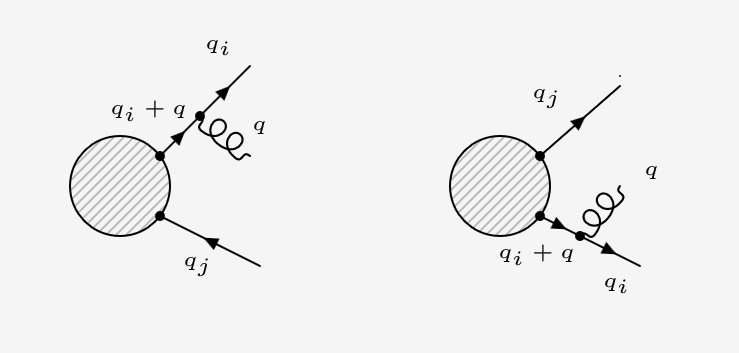
\includegraphics[width=0.85\textwidth]{images/qqg-diagrams.png}
\end{figure}

\subsection{qg-$\bar{q}$}

\begin{figure}[h!]
\centering
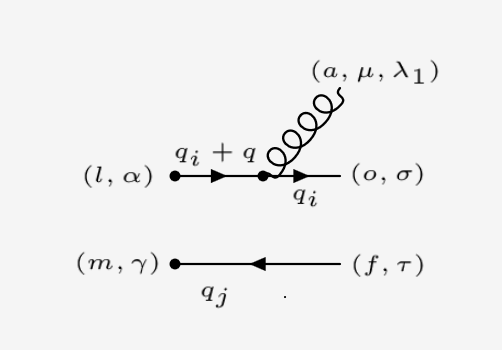
\includegraphics[scale=0.7]{images/qgqbarM.png}
\end{figure}

\begin{equation}
M_1 = [{\bar{u}}_{\sigma}(q_i) (-ig_s \gamma^{\mu}\times {[T^a]_o}^l)  \frac{i(\not{q_i} + \not{q})}{(q_i + q)^2} {\varepsilon^{\lambda_1}}_{\mu} (q)]\: [{v}_{\tau}(q_j)]
\end{equation}
\pagebreak
\begin{figure}[h!]
\centering
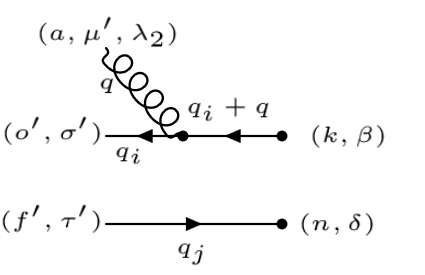
\includegraphics[scale=0.7]{images/qgqbarMDega.png}
\end{figure}

\begin{equation}
{M_1}^{\dagger} = [\frac{-i(\not{q_i} + \not{q})}{(q_i + q)^2} \:  (ig_s \gamma^{{\mu}^{\prime}}\times {[T^b]_{o\:^{\prime}}}^k) \: u_{{\sigma}^{\prime}}(q_i) \: {\varepsilon^{\lambda_2}}_{{\mu}^{\prime}} (q)][{\bar{v}}_{{\tau}^{\prime}}(q_j)]
\end{equation}

\begin{figure}[h!]
\centering
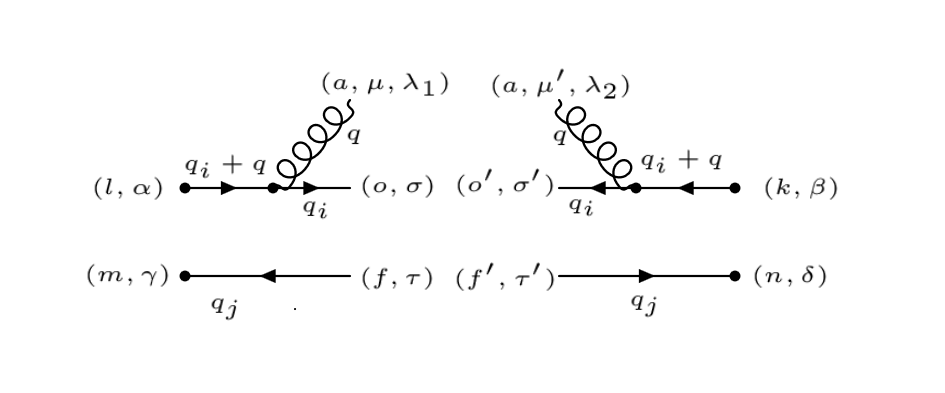
\includegraphics[width=0.85\textwidth]{images/qgqbarMSquer.png}
\end{figure}

\begin{equation}
\begin{split}
|M_1|^2=M_1\:{\color[RGB]{255,0,0} {M_1}^{\dagger}} = [{\bar{u}}_{\sigma}(q_i)\: (-ig_s \gamma^{\mu}\times {[T^a]_o}^l) \: \frac{i(\not{q_i} + \not{q})}{(q_i + q)^2}\:\: {\varepsilon^{\lambda_1}}_{\mu} (q)] [{v}_{\tau}(q_j)]\: \\
\quad\quad\quad\quad\quad\quad\quad\quad\:\:{\color[RGB]{255,0,0}[\frac{-i(\not{q_i} + \not{q})}{(q_i + q)^2} \:  (ig_s \gamma^{{\mu}^{\prime}}\times {[T^b]_{o\:^{\prime}}}^k) \: u_{{\sigma}^{\prime}}(q_i) \: {{\varepsilon^{\lambda_2}}_{{\mu}^{\prime}}}^* (q)][{\bar{v}}_{{\tau}^{\prime}}(q_j)]}
\end{split}
\end{equation}


\begin{equation}
\begin{split}
|M_1|^2=[\frac{-i(\not{q_i} + \not{q})}{(q_i + q)^2} \:
 \:  (ig_s \gamma^{{\mu}^{\prime}}\times {[T^b]_{o\:^{\prime}}}^k) \: {\bar{u}}_{\sigma}(q_i)\:u_{{\sigma}^{\prime}}(q_i) \: {{\varepsilon^{\lambda_2}}_{{\mu}^{\prime}}^* (q) {\varepsilon^{\lambda_1}}_{\mu} (q)} \\
\times (-ig_s \gamma^{\mu}\times {[T^a]_o}^l) \: \frac{i(\not{q_i} + \not{q})}{(q_i + q)^2} ]
[{\bar{v}}_{{\tau}^{\prime}}(q_j) {v}_{\tau}(q_j)]
\end{split}
\end{equation}

and after sum over the lorenz index $({\sigma},{\sigma}^{\prime})$ and $({\tau},{\tau}^{\prime})$ and unsing the spin addition relation:
 
\begin{equation}
\begin{split}
\displaystyle\sum\limits_{{\sigma},{\sigma}^{\prime}} {\bar{u}}_{\sigma}(q_i)\:u_{{\sigma}^{\prime}}(q_i) = \not{q_i},\\
\displaystyle\sum\limits_{{\tau},{\tau}^{\prime}} {\bar{v}}_{\tau}(q_j)\:v_{{\tau}^{\prime}}(q_j) = \not{q_j}
\end{split}
\end{equation}
and sum over polarization index $({\lambda_{1}},{\lambda}_{2})$ :
\begin{equation}
\begin{split}
 \displaystyle\sum\limits_{{\mu},{\mu}^{\prime}} {{\varepsilon^{\lambda_2}}_{{\mu}^{\prime}}^* (q) {\varepsilon^{\lambda_1}}_{\mu} (q)} = -g_{{\mu}{\mu}^{\prime}}
\end{split}
\end{equation}

\begin{equation}
\begin{split}
|M_1|^2=\frac{-g_s^2  {[T^b]_{o\:^{\prime}}}^k \: {[T^a]_o}^l }{(q_i + q)^2 (q_i + q)^2}
[(\not{q_i} + \not{q}) \:
 \:  \gamma^{{\mu}^{\prime}} \: \not{q_i} \: g_{{{\mu}^{\prime}}{\mu}} 
\gamma^{\mu} \: (\not{q_i} + q)]
[\not{q_j}]
\end{split}
\end{equation}

from here and after contraction between all indices we can actually make statements about the last result.
\begin{equation}
\begin{split}
|M_1|^2=\frac{-g_s^2  {[T^b]_{o\:^{\prime}}}^k \: {[T^a]_o}^l }{(q_i + q)^2 (q_i + q)^2}
[(\not{q_i} + \not{q}) \:
 \:  \gamma^{{\mu}^{\prime}} \: \not{q_i} \: 
\gamma_{{\mu}^{\prime}} \: (\not{q_i} + q)]
[\not{q_j}]
\end{split}
\end{equation}

In other words we expect the tree level diagram from LO and a number:
\begin{figure}[h!]
\centering
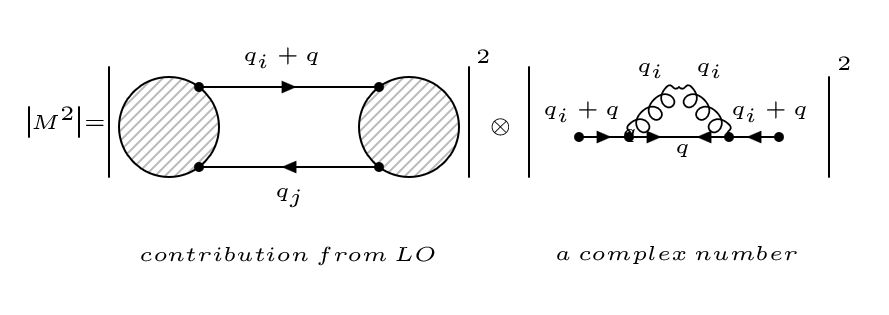
\includegraphics[width=0.85\textwidth]{images/expectationqg-qbar.png}
\end{figure}
Which means:\\
\begin{equation}
\begin{split}
|M_1|^2=\frac{-g_s^2  {[T^b]_{o\:^{\prime}}}^k \: {[T^a]_o}^l }{(q_i + q)^2 (q_i + q)^2}
[\not{P_i}]
[\not{P_j}]\:\otimes \: {\color[RGB]{255,0,0} (a\: complex\: number)}
\end{split}
\end{equation}  
Let's calculate the contribution and compare the final result with this expectation:
\begin{equation}
\begin{split}
N=: \gamma^{{\mu}^{\prime}} \not{q_i} \: \gamma_{{\mu}^{\prime}} = {q_{i\sigma}} \: \gamma^{{\mu}^{\prime}} \gamma^{\sigma} \:\: \gamma_{{\mu}^{\prime}}\\
={q_{i\sigma}} \: (\lbrace{\gamma^{{\mu}^{\prime}}}, {\gamma^{\sigma}}\rbrace \: - {\gamma^{\sigma}}{\gamma^{{\mu}^{\prime}}})\gamma_{{\mu}^{\prime}}\\
={q_{i\sigma}} \: 2g^{{{\mu}^{\prime}}{\sigma}} \: \gamma_{{\mu}^{\prime}} \: - \:d\:{\gamma^{\sigma}}\\
=(2-d) \not{q_i}
\end{split}
\end{equation}

\begin{equation}
\begin{split}
|M_1|^2=-(2-d)\:\frac{g_s^2  {[T^b]_{o\:^{\prime}}}^k \: {[T^a]_o}^l }{(q_i + q)^2 (q_i + q)^2}
[(\not{q_i} + \not{q}) \:
 \:\not{q_i} \: 
 \: (\not{q_i} + q)]
[\not{q_j}]
\end{split}
\end{equation}

\begin{equation}
\begin{split}
|M_1|^2=-(2-d)\:\frac{g_s^2  {[T^b]_{o\:^{\prime}}}^k \: {[T^a]_o}^l }{(q_i + q)^2 (q_i + q)^2}
[\not{q_i} \not{q_i} \not{q_i} \: + \: \not{q_i} \not{q_i} \not{q} \: + \: \not{q} \not{q_i} \not{q_i} \:+\: \not{q} \not{q_i} \not{q}]
[\not{q_j}]
\end{split}
\end{equation}

For the momenta are on-shell which means:
\begin{equation}
\begin{split}
\not{q_i}\not{q_i} = {q_i}= m^2\\
\not{q}\not{q} = {q}= m^2\\
\not{q_j}\not{q_j} = {q_j}= m^2
\end{split}
\end{equation}

we can first neglect the mass of patrons and ignore each term with $ \not{q_i}\not{q_i} $ and  $ \not{q}\not{q} $ as well.

\begin{equation}
\begin{split}
|M_1|^2=-(2-d)\:\frac{g_s^2  {[T^b]_{o\:^{\prime}}}^k \: {[T^a]_o}^l }{(2q_i q)(2q_i q)}
[\not{q} \not{q_i} \not{q}]
[\not{q_j}]
\end{split}
\end{equation}

\begin{equation}
\begin{split}
L=\not{q} \not{q_i} \not{q} =\not{q}[{q_{i\sigma}} q_{\mu} \: (\lbrace{\gamma^{\mu}}, {\gamma^{\sigma}}\rbrace - {\gamma^{\sigma}}{\gamma^{\mu}})]\\ 
\not{q}[2{q_{i}}^{\mu} q_{\mu} - {q_{i\sigma}}q_{\mu}{\gamma^{\mu}}{\gamma^{\sigma}}\\
=\not{q} (2q_i q)-q_{\mu}{q_{i\sigma}}q_{\mu}[{\gamma^{\mu}}{\gamma^{\mu}}{\gamma^{\sigma}}]\\
=\not{q} (2q_i q)-q_{\mu}{q_{i\sigma}}q_{\mu}[\frac{{\gamma^{\mu}}{\gamma^{\mu}}}{2} +\frac{{\gamma^{\mu}}{\gamma^{\mu}}}{2}]{\gamma^{\sigma}}\\
=\not{q} (2q_i q)-q_{\mu}{q_{i\sigma}}q_{\mu}[g^{{\mu}{\mu}}]{\gamma^{\sigma}}\\
=\not{q} (2q_i q)-q_{\mu}{q_{i\sigma}}q^{\mu}{\gamma^{\sigma}}\\
=\not{q} (2q_i q)-q^2 \not{q_i}\\
=\not{q}
\end{split}
\end{equation}
After inserting the last result of $ L $ and simplify the term $ (2q_i q) $ from the denominator and nominator because , we get:
\begin{equation}
\begin{split}
|M_1|^2=-(2-d)\:\frac{g_s^2  {[T^b]_{o\:^{\prime}}}^k \: {[T^a]_o}^l }{(2q_i q)}
[\not{q_i}]
[\not{q_j}]
\end{split}
\end{equation}
Now we are going to use the parametrisation from equation (1) to reduce the 3-member matrix element to 2-member and take out the singularity term from the amplitude.
\begin{equation}
\begin{split}
|M_1|^2=(d-2)\:\frac{g_s^2  {[T^b]_{o\:^{\prime}}}^k \: {[T^a]_o}^l }{(2q_i q)}
[(1-z) \not{p_i}+zy \not{p_j} - \sqrt{zy(1-z)} \not{{m}_{\bot}}] \not{{m}_{\bot}}]
[(1-y) \not{{p_j}^{\mu}}]
\end{split}
\end{equation}
Multiplying the both sides 
\begin{equation}
\begin{split}
|M_1|^2=(d-2)\:\frac{g_s^2  {[T^b]_{o\:^{\prime}}}^k \: {[T^a]_o}^l }{(2q_i q)}
[(1-z)(1-y) \not{p_i}\not{p_j} \\
+zy(1-y) \not{p_j}\not{p_j} + (1-y)\sqrt{zy(1-z)} \not{{m}_{\bot}}\not{p_j}]
\end{split}
\end{equation}
and under consideration of the fact that $ p_i $ and $ p_j $ are the on-shell momenta of the emitter and spectator partons, we can ignore the terms with $ \not{p_i} \not{p_i} $ and $ \not{p_j} \not{p_j} $.
The $ {p_i} \cdot  {m}_{\bot} $ and $ {p_j} \cdot  {m}_{\bot} $ are always $ 0 $ because the $ p_i $ and $ p_j $ are lightlike, i.e. zero transverse component. So those terms can be neglected.


\begin{equation}
\begin{split}
|M_1|^2=(d-2)(1-z)(1-y)\:\frac{g_s^2  {[T^b]_{o\:^{\prime}}}^k \: {[T^a]_o}^l }{(2q_i q)}
[\not{p_i}][\not{p_j}]
\end{split}
\end{equation}
\newpage

\subsection{$\bar{q}$g-q}

\begin{figure}[h!]
\centering
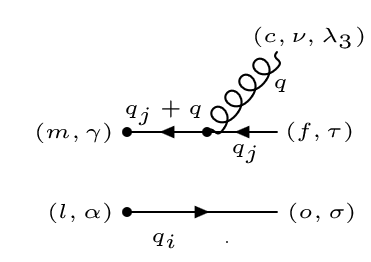
\includegraphics[scale=0.7]{images/qbargqM.png}
\end{figure}

\begin{equation}
M_2 = [\frac{i(\not{q_i} + \not{q})}{(q_i + q)^2} (-ig_s \gamma^{\nu}\times {[T^c]_f}^m) \:{v}_{\tau}(q_i)\: {\varepsilon^{\lambda_3}}_{\nu} (q)]\: [{u}_{\sigma}(q_j)]
\end{equation}
\begin{figure}[h!]
\centering
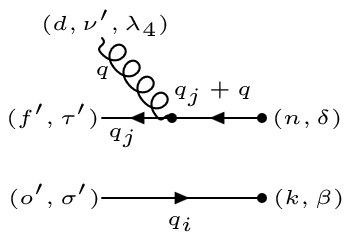
\includegraphics[scale=0.7]{images/qbargqMDega.png}
\end{figure}
\begin{equation}
M_2^{\dagger} = [\bar{v}_{{\tau}^{\prime}}(q_i) \: (ig_s \gamma^{{\nu}^{\prime}}\times {[T^d]_{f^{\prime}}}^n) \: \frac{-i(\not{q_i} + \not{q})}{(q_i + q)^2} \: {\varepsilon^{\lambda_4}}_{{\nu}^{\prime}} (q)]\: [\bar{u}_{{\sigma}^{\prime}}(q_j)]
\end{equation}

\begin{figure}[h!]
\centering
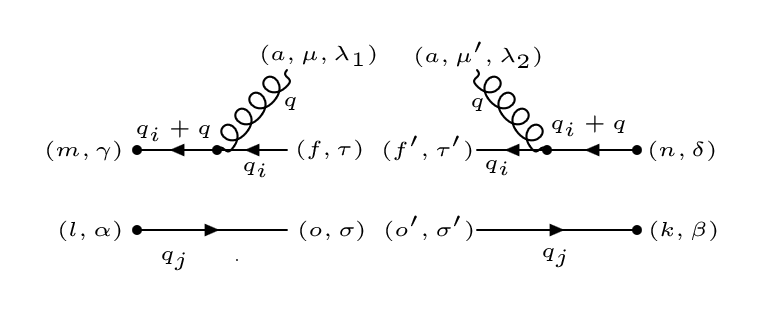
\includegraphics[width=0.85\textwidth]{images/qbargqMSquer.png}
\end{figure}

\begin{equation}
\begin{split}
|M_2|^2=M_2\:{\color[RGB]{255,0,0} {M_2}^{\dagger}} = [\frac{i(\not{q_i} + \not{q})}{(q_i + q)^2} (-ig_s \gamma^{\nu}\times {[T^c]_f}^m) \:{v}_{\tau}(q_i)\: {\varepsilon^{\lambda_3}}_{\nu} (q)]\: [{u}_{\sigma}(q_j)]\: \\
\quad\quad\quad\quad\quad\quad\quad\quad\:\:{\color[RGB]{255,0,0}[\bar{v}_{{\tau}^{\prime}}(q_i) \: (ig_s \gamma^{{\nu}^{\prime}}\times {[T^d]_{f^{\prime}}}^n) \: \frac{-i(\not{q_i} + \not{q})}{(q_i + q)^2} \: {\varepsilon^{\lambda_4}}_{{\nu}^{\prime}} (q)]\: [\bar{u}_{{\sigma}^{\prime}}(q_j)]}
\end{split}
\end{equation}


\begin{equation}
\begin{split}
|M_2|^2 =\frac{g_s^2 \: {[T^c]_f}^m \: {[T^d]_{f^{\prime}}}^n }{(q_i + q)^2 (q_i + q)^2} [(\not{q_i} + \not{q}) \gamma^{\nu}  \:{v}_{\tau}(q_i)\bar{v}_{{\tau}^{\prime}}(q_i)\: {\varepsilon^{\lambda_3}}_{\nu} (q){\varepsilon^{\lambda_4}}_{{\nu}^{\prime}}  (q) \gamma^{{\nu}^{\prime}}(\not{q_i} + \not{q})]\: \\
[{u}_{\sigma}(q_j) ]
\: [\bar{u}_{{\sigma}^{\prime}}(q_j)]
\end{split}
\end{equation}

and after sum over the lorenz index $({\sigma},{\sigma}^{\prime})$ and $({\tau},{\tau}^{\prime})$ and unsing the spin addition relation:
 
\begin{equation}
\begin{split}
\displaystyle\sum\limits_{{\sigma},{\sigma}^{\prime}} {\bar{u}}_{\sigma}(q_j)\:u_{{\sigma}^{\prime}}(q_j) = \not{q_j},\\
\displaystyle\sum\limits_{{\tau},{\tau}^{\prime}} {\bar{v}}_{\tau}(q_i)\:v_{{\tau}^{\prime}}(q_i) = \not{q_i}
\end{split}
\end{equation}
and sum over polarization index $({\lambda_{3}},{\lambda}_{4})$ :
\begin{equation}
\begin{split}
 \displaystyle\sum\limits_{{\nu},{\nu}^{\prime}} {{\varepsilon^{\lambda_4}}_{{\nu}^{\prime}}^* (q) {\varepsilon^{\lambda_3}}_{\nu} (q)} = -g_{{\nu}{\nu}^{\prime}}
\end{split}
\end{equation}

\begin{equation}
\begin{split}
|M_2|^2 =\frac{g_s^2 \: {[T^c]_f}^m \: {[T^d]_{f^{\prime}}}^n }{(q_i + q)^2 (q_i + q)^2} [(\not{q_i} + \not{q}) \gamma^{\nu}  \:\not{q_i}\: (-g_{{\nu}{{\nu}^{\prime}}}) \gamma^{{\nu}^{\prime}}(\not{q_i} + \not{q})]\: 
[\not{q_j} ]
\end{split}
\end{equation}

After the same calculation from the last part, we'll get:

\begin{equation}
\begin{split}
|M_2|^2 =(d-2) \frac{g_s^2 \: {[T^c]_f}^m \: {[T^d]_{f^{\prime}}}^n }{(2qq_i)} [\not{q}]\: 
[\not{q_j} ]
\end{split}
\end{equation}

In this case we have to be careful because the quark is the emitter and we have to insert the right parametrisation for this, namely: 
\begin{equation}
	{q_j}^{\mu} = z{p_i}^{\mu} + y(1-z){p_j}^{\mu} + \sqrt{zy(1-z)}{m}_{\bot}
\end{equation}
To avoid such irritating problems we ought to compute this matrix element with the exact same initialized  $ i, j $ from $ |M_1|^2 $. But it's also possible to do that in reverse order as far as we know what we do. After parametrisation we'll get:
\begin{equation}
\begin{split}
|M_2|^2 =(d-2) \frac{g_s^2 \: {[T^c]_f}^m \: {[T^d]_{f^{\prime}}}^n }{(2qq_i)} 
[z \not{p_i}+y(1-z) \not{p_j} + \sqrt{zy(1-z)} \not{{m}_{\bot}}]\\
[z\not{p_i} + y(1-z)\not{p_j} + \sqrt{zy(1-z)}\not{m}_{\bot}]
\end{split}
\end{equation}
Multiplying the both side gives:

\begin{equation}
\begin{split}
|M_2|^2 =(d-2) \frac{g_s^2 \: {[T^c]_f}^m \: {[T^d]_{f^{\prime}}}^n }{(2qq_i)} 
[(1-z) \not{p_i}+zy \not{p_j} - \sqrt{zy(1-z)} \not{{m}_{\bot}}]\\
[z\not{p_i} + y(1-z)\not{p_j} + \sqrt{zy(1-z)}\not{m}_{\bot}]
\end{split}
\end{equation}


\begin{equation}
\begin{split}
\Longrightarrow|M_2|^2 =(d-2) \frac{g_s^2 \: {[T^c]_f}^m \: {[T^d]_{f^{\prime}}}^n }{(2qq_i)}
[(1-z)z \not{p_i}\not{p_i} + y(1-z)^2 \not{p_i}\not{p_j}\\
+(1-z)  \sqrt{zy(1-z)} \not{p_i}\not{m}_{\bot}+z^2y \not{p_j}\not{p_i} + zy^2 (1-y)\not{p_j}\not{p_j}+zy \sqrt{zy(1-z)} \not{p_j} \not{{m}_{\bot}}\\
- z\sqrt{zy(1-z)} \not{{m}_{\bot}}\not{p_i}-y(1-z) \sqrt{zy(1-z)} \not{{m}_{\bot}}\not{p_j}-zy(1-z) \not{{m}_{\bot}}\not{{m}_{\bot}}]
\end{split}
\end{equation}

\begin{equation}
\begin{split}
\Longrightarrow|M_2|^2 =(d-2) \frac{g_s^2 \: {[T^c]_f}^m \: {[T^d]_{f^{\prime}}}^n }{(2qq_i)}
[y(1-z)^2 \not{p_i}\not{p_j}
+z^2y \not{p_j}\not{p_i}]
\end{split}
\end{equation}

we're changing the position of two matrices to be able to sum the coefficients 
\begin{equation}
\not{p_j}\not{p_i} = -\not{p_i}\not{p_j}
\end{equation} 

\begin{equation}
\begin{split}
\Longrightarrow|M_2|^2 =(d-2) \frac{g_s^2 \: {[T^c]_f}^m \: {[T^d]_{f^{\prime}}}^n }{(2qq_i)}
[y(1-z)^2 \not{p_i}\not{p_j}
-z^2y \not{p_i}\not{p_j}]
\end{split}
\end{equation}
finally:
\begin{equation}
\begin{split}
\Longrightarrow|M_2|^2 =(d-2)y(1-2z) \frac{g_s^2 \: {[T^c]_f}^m \: {[T^d]_{f^{\prime}}}^n }{(2qq_i)}
[\not{p_i}\not{p_j}
]
\end{split}
\end{equation}


\newpage

\subsection{$M_1 {M_2}^{\dagger}$}

\begin{figure}[h!]
\centering
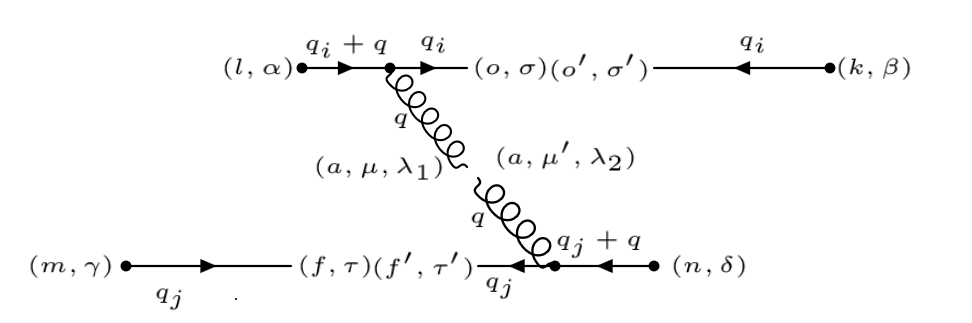
\includegraphics[width=0.85\textwidth]{images/M1M2Degaqqg.png}
\end{figure}

\subsection{$|M^{2}|$}

\begin{figure}[h!]
\centering
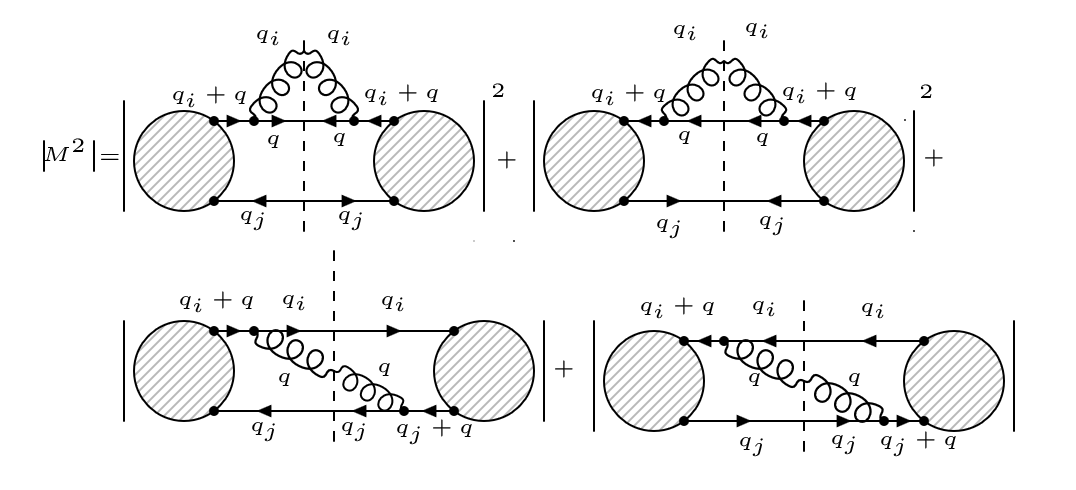
\includegraphics[width=0.85\textwidth]{images/qqgMSquer.png}
\end{figure}

\begin{figure}[h!]
\centering
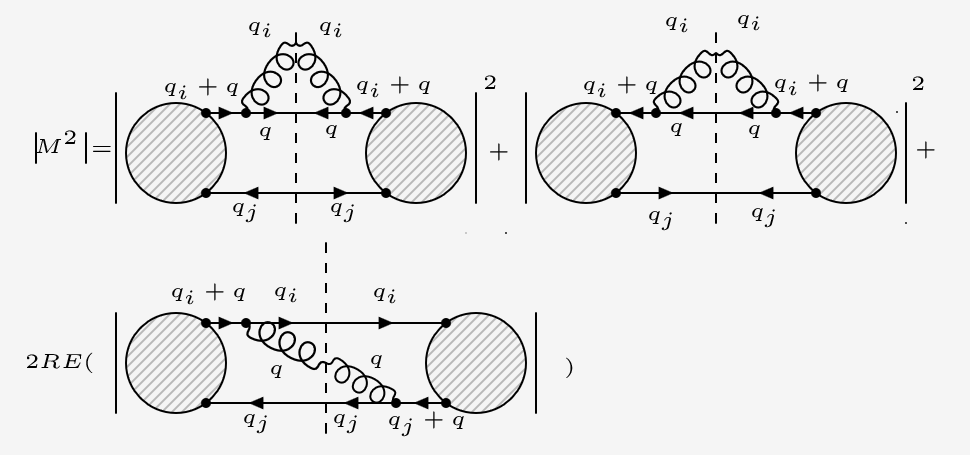
\includegraphics[width=0.85\textwidth]{images/REqqgMSquer.png}
\end{figure}

\newpage